\setlength{\parskip}{\baselineskip}
\section{FPGA Implementation}

\begin{frame}
    \huge FPGA Implementation
\end{frame}

% Todo: Replace with your platform
\begin{frame}{Xilinx ZCU102 Evaluation Kit}
	\begin{minipage}{0.6\textwidth}
    	\centering
    	\includegraphics[width=1\textwidth]{../Images/Hardware/ZCU102-board-overview.jpg}\\
	\end{minipage}%
	\begin{minipage}{0.4\textwidth}
		\begin{itemize}
		    \item SoC with ARM CPU
	        \item Multiple peripherals
	        \item Great for prototyping edge applications
		\end{itemize}
	\end{minipage}
\end{frame}

% \begin{frame}{Tools Used: Vitis Unified Software Platform}
% 	\begin{minipage}{0.6\textwidth}
% 		\centering
% 		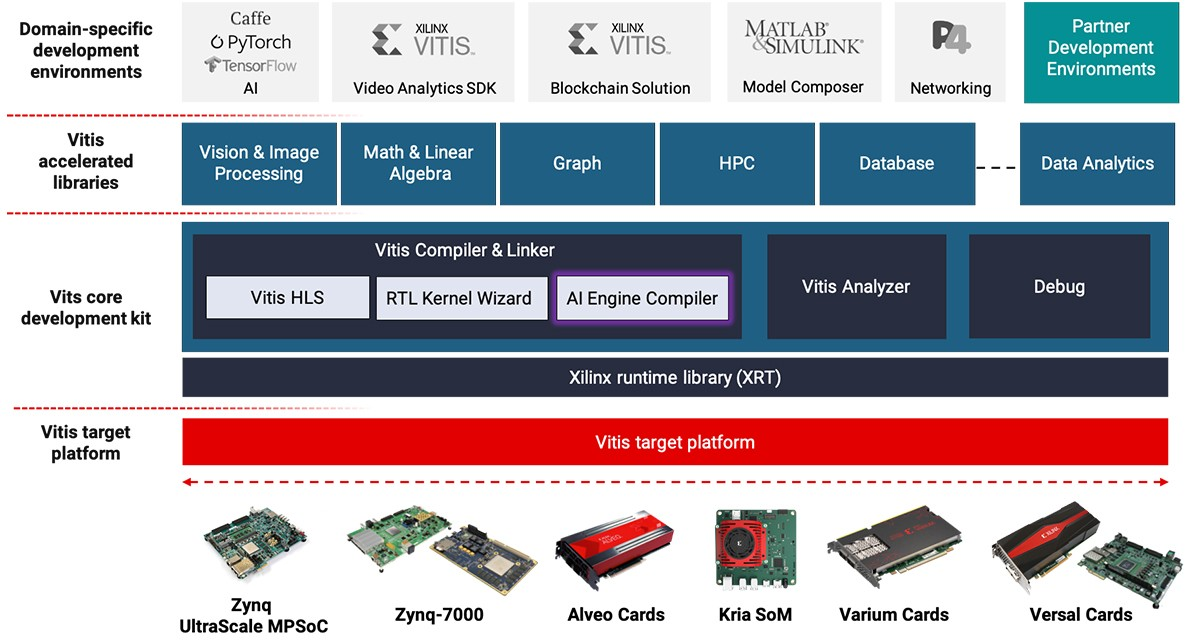
\includegraphics[width=1\textwidth]{Images/Platform/vitis.jpg}\\
% 	\end{minipage}%
% 	\begin{minipage}{0.4\textwidth}
% 		\begin{itemize}
% 			\item tools, libraries
% 			\item compilers, debuggers
% 			\item analyze \& profile designs
% 			\item support HDL and HLS
% 		\end{itemize}
% 	\end{minipage}
% \end{frame}

% \begin{frame}{Tools Used: Vitis Unified Software Platform}
% 	\begin{minipage}{0.6\textwidth}
% 		\centering
% 		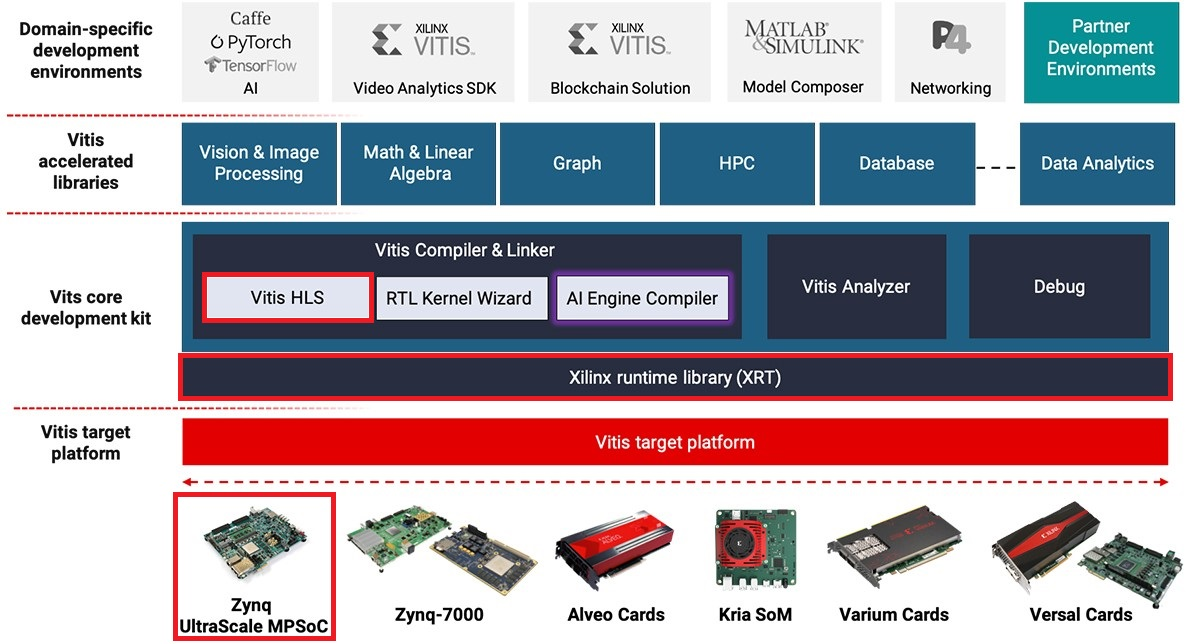
\includegraphics[width=1\textwidth]{Images/Platform/vitis_highlited.jpg}\\
% 	\end{minipage}%
% 	\begin{minipage}{0.4\textwidth}
% 		\begin{itemize}
% 			\item tools, libraries
% 			\item compilers, debuggers
% 			\item analyze \& profile designs
% 			\item support HDL and HLS
% 		\end{itemize}
% 	\end{minipage}
% \end{frame}

\begin{frame}{Tools Used: Vitis High Level Synthesis (HLS)}
	\begin{itemize}
	    \item Synthesize "C/C++ like" code to RTL
	    \item Automate large parts of the implementations
	    \item Provide optimized libraries for data types, interfaces, etc.
	\end{itemize}\\
	\begin{table}[H]
        \center
        \small
        \begin{tabular}{ | c | }
            \hline
            Designer's Responsibilities\\
            \hline
            Macro Architecture\\
            Design Intent\\
            Constrains\\
            \hline
            \multicolumn{1}{ c }{ } \\
            \multicolumn{1}{ c }{ } \\
            \multicolumn{1}{ c }{ } \\
            \multicolumn{1}{ c }{ } \\
        \end{tabular}
        \quad
        \begin{tabular}{ | c | }
            \hline
            HLS tool automation\\
            \hline
            FSM Generation\\
            Operation Scheduling\\
            Clock\\
            Register Pipelining\\
            Resource Sharing\\
            Timing\\
            Verification\\
            \hline
        \end{tabular}
        \caption*{Distribution of work during HLS design.}
    \end{table}
\end{frame}

\begin{frame}{Xilinx Runtime library (XRT)}
	\begin{itemize}
	    \item Facilitate communication between PS \& PL
	    \item Manage shared memory
	    \item Portable \& open-source % portability can be used to transfer to heterogeneous devices
	\end{itemize}\\
	\begin{figure}[H]
            \centering
		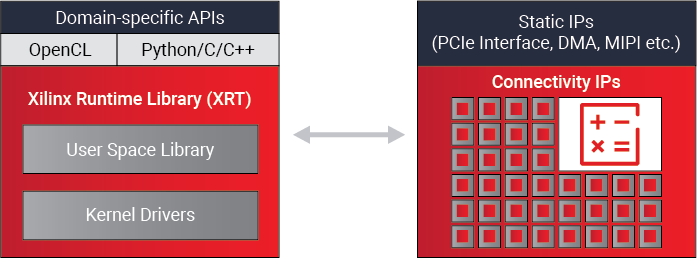
\includegraphics[width=0.6\textwidth]{Images/Platform/xrt.png}
	\end{figure}%
\end{frame}

% \begin{frame}{Embedded Systems Perspective}
% % 	\begin{minipage}{0.6\textwidth}
%     	\begin{figure}[H]
%             \centering
%     		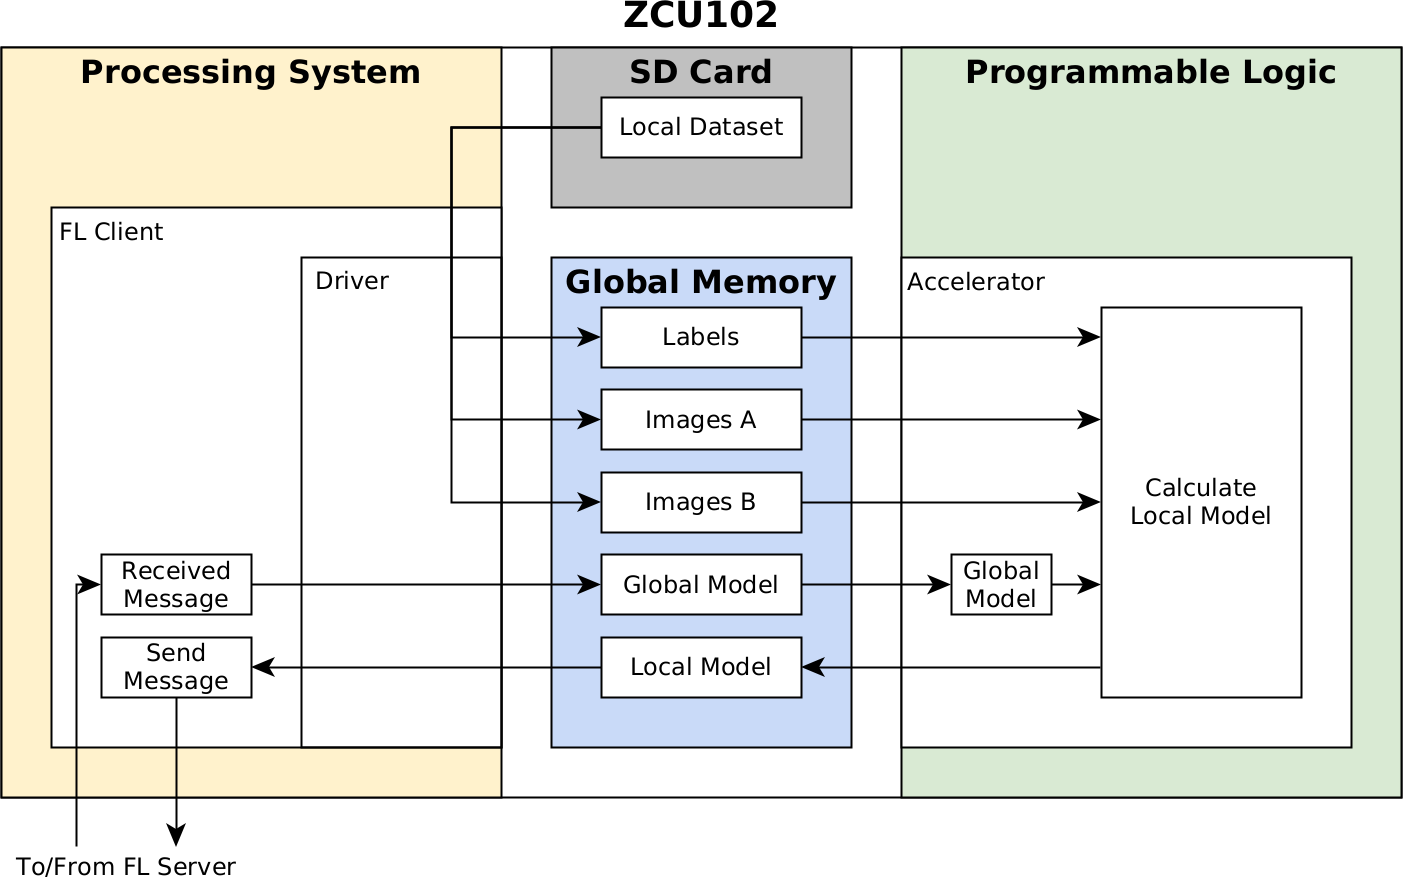
\includegraphics[height=0.8\textheight]{Images/Diagrams/zcu_FL_client.png}
%     	\end{figure}%
% % 	        FL client from chapter 4\\
% % 	        Using Linux sockets\\
% % 	        Driver (XRT) manages Global Memory \& Accelerator\\
% % 	        Accelerator created with HLS\\
% % 	\end{minipage}%
% \end{frame}

\begin{frame}{CPU-based C++ CNN implementation}
    % Discover the flow of the data in the design.
	\begin{minipage}{0.6\textwidth}
    	\begin{figure}[H]
            \centering
    		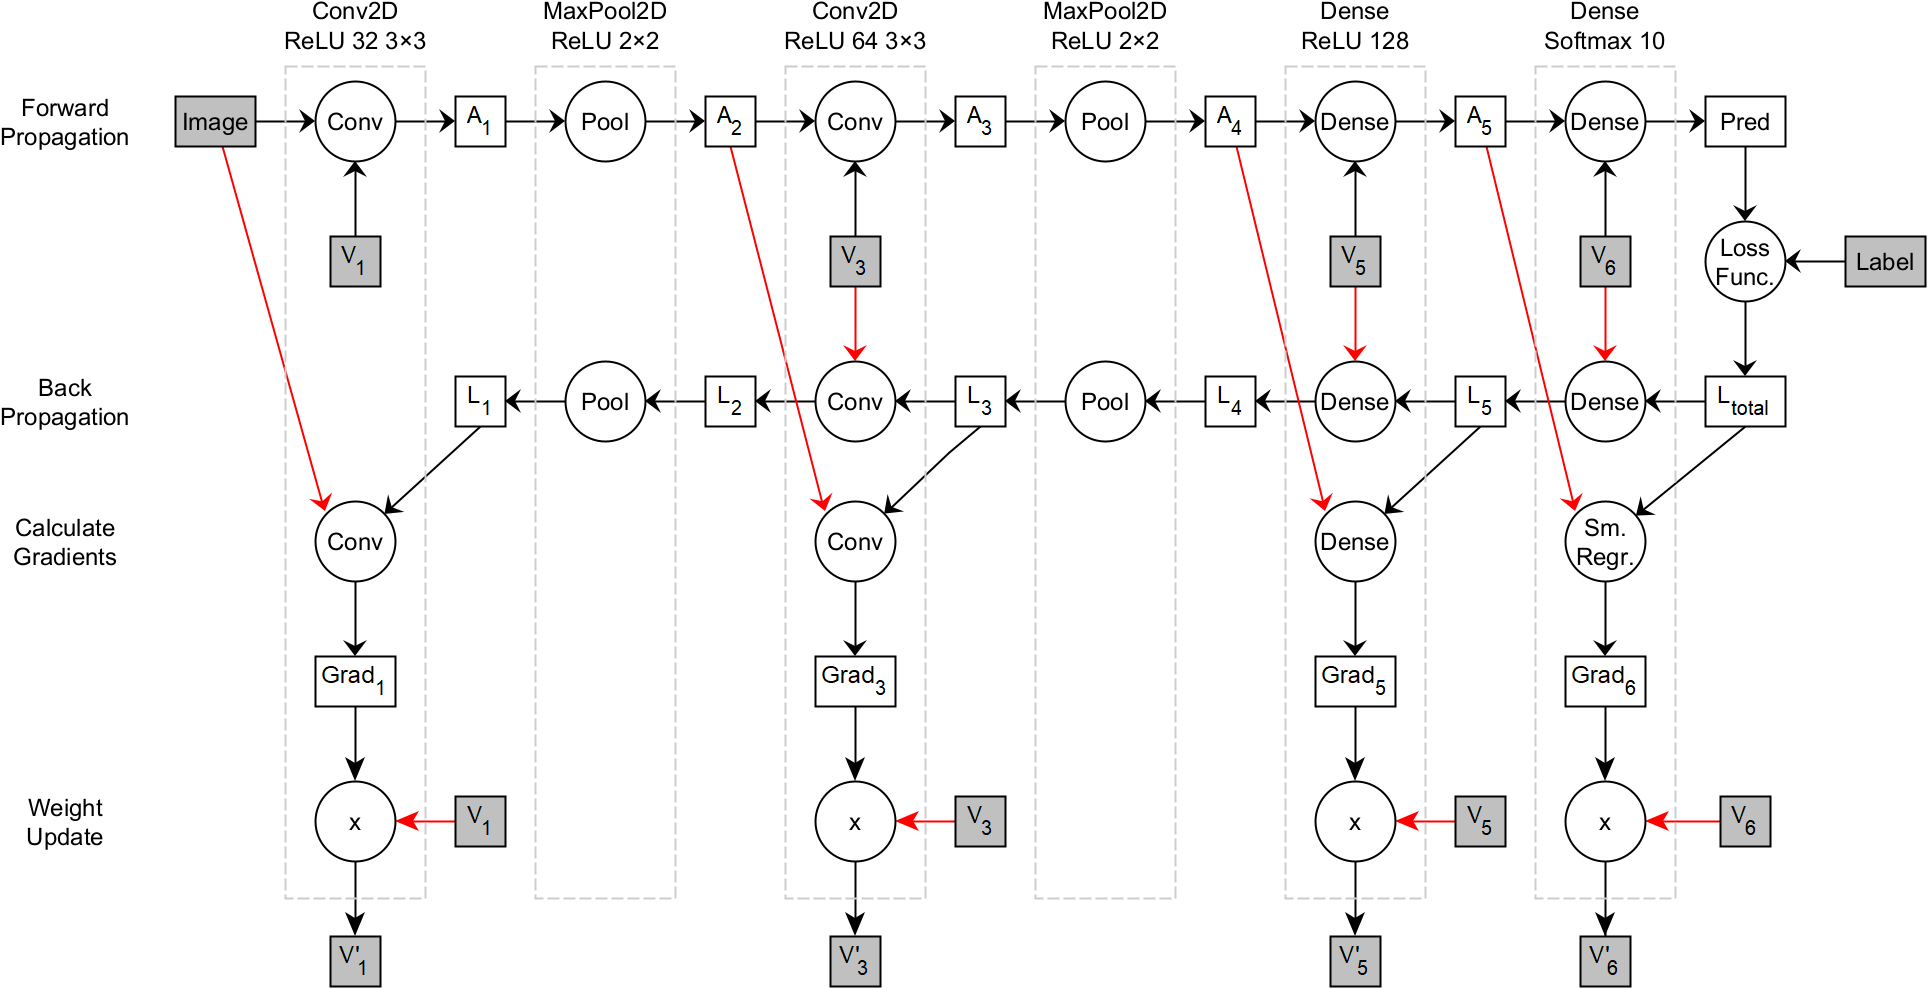
\includegraphics[width=1\textwidth]{Images/Diagrams/dataflow_cnn_model.png}
            \caption*{Dataflow diagram of the implemented CNN}
    	\end{figure}%
	\end{minipage}%
	\begin{minipage}{0.4\textwidth}
    	\vspace{1cm}
    	\begin{itemize}
    	    \item 6 layers \& $\sim$105000 variables
    	    \item Convolutional, max-pooling \& dense layers
    	    \item ReLU \& Softmax Activations
    	    \item Float32 implementation
    	\end{itemize}
	\end{minipage}%
\end{frame}
% works as map for the development of the HLS implementation
% enable logging of all data for verification of HLS implementation
% discover the flow of the data, data that skip functions will require special attention
% softmax is a barrier. To be calculated, everything before it must be calculated first

\begin{frame}{FPGA-based CNN implementation - 2D Convolutional Layers- Access Pattern}
	\begin{minipage}{0.45\textwidth}
    	\begin{figure}[H]
            \centering
    		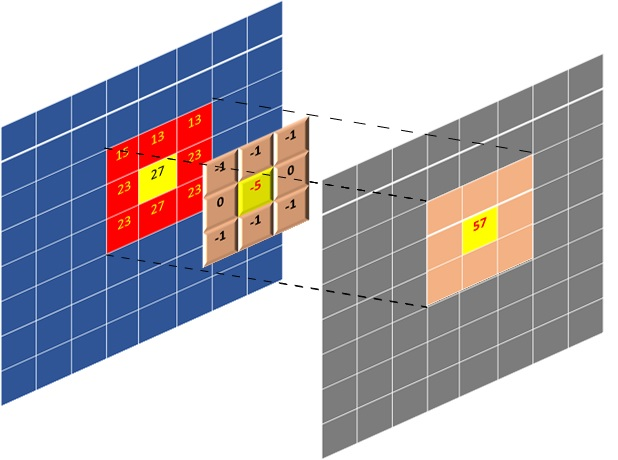
\includegraphics[width=1\textwidth]{Images/Diagrams/convolution_access_pattern.jpg}
            \caption*{Data access patern of 2D convolution}
    	\end{figure}%
	\end{minipage}%
	\begin{minipage}{0.55\textwidth}
    	\begin{itemize}
    	    \item Input pixels are accessed serially
    	    \item Two dimensional filters with non-serial access pattern
    	    \item Input pixels have to be reused
    	    \item Float32 implementation
    	\end{itemize}
	\end{minipage}%
\end{frame}

\begin{frame}{FPGA-based CNN implementation - 2D Convolutional Layers - Line Buffers}
	\begin{minipage}{0.5\textwidth}
    	\begin{figure}[H]
            \centering
    		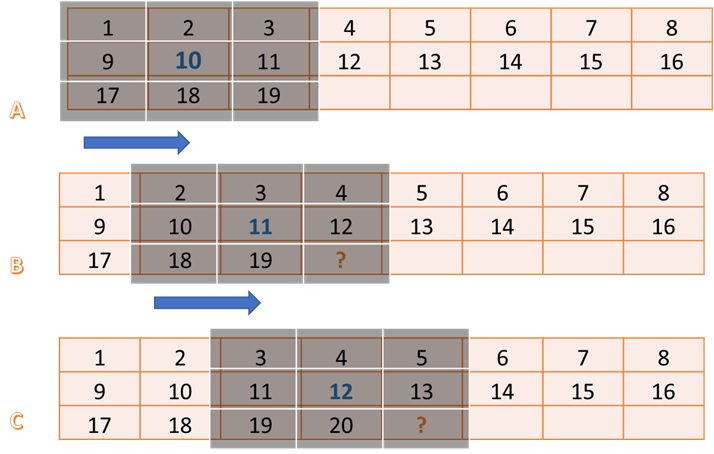
\includegraphics[width=1\textwidth]{Images/Diagrams/line_buf_conv.jpg}
            \caption*{Line Buffers with 3$\times$3 windows}
    	\end{figure}%
	\end{minipage}%
	\begin{minipage}{0.5\textwidth}
    	\begin{itemize}
    	    \item Write input pixels serially
    	    \item Access them through 3$\times$3 windows with stride 1
    	    \item Padding required
    	    \item Expandable for multiple input channels
    	\end{itemize}
	\end{minipage}%
\end{frame}

\begin{frame}{FPGA-based CNN implementation - 2D Convolutional Layers - Computations}
	\begin{minipage}{0.4\textwidth}
    	\begin{figure}[H]
            \centering
    		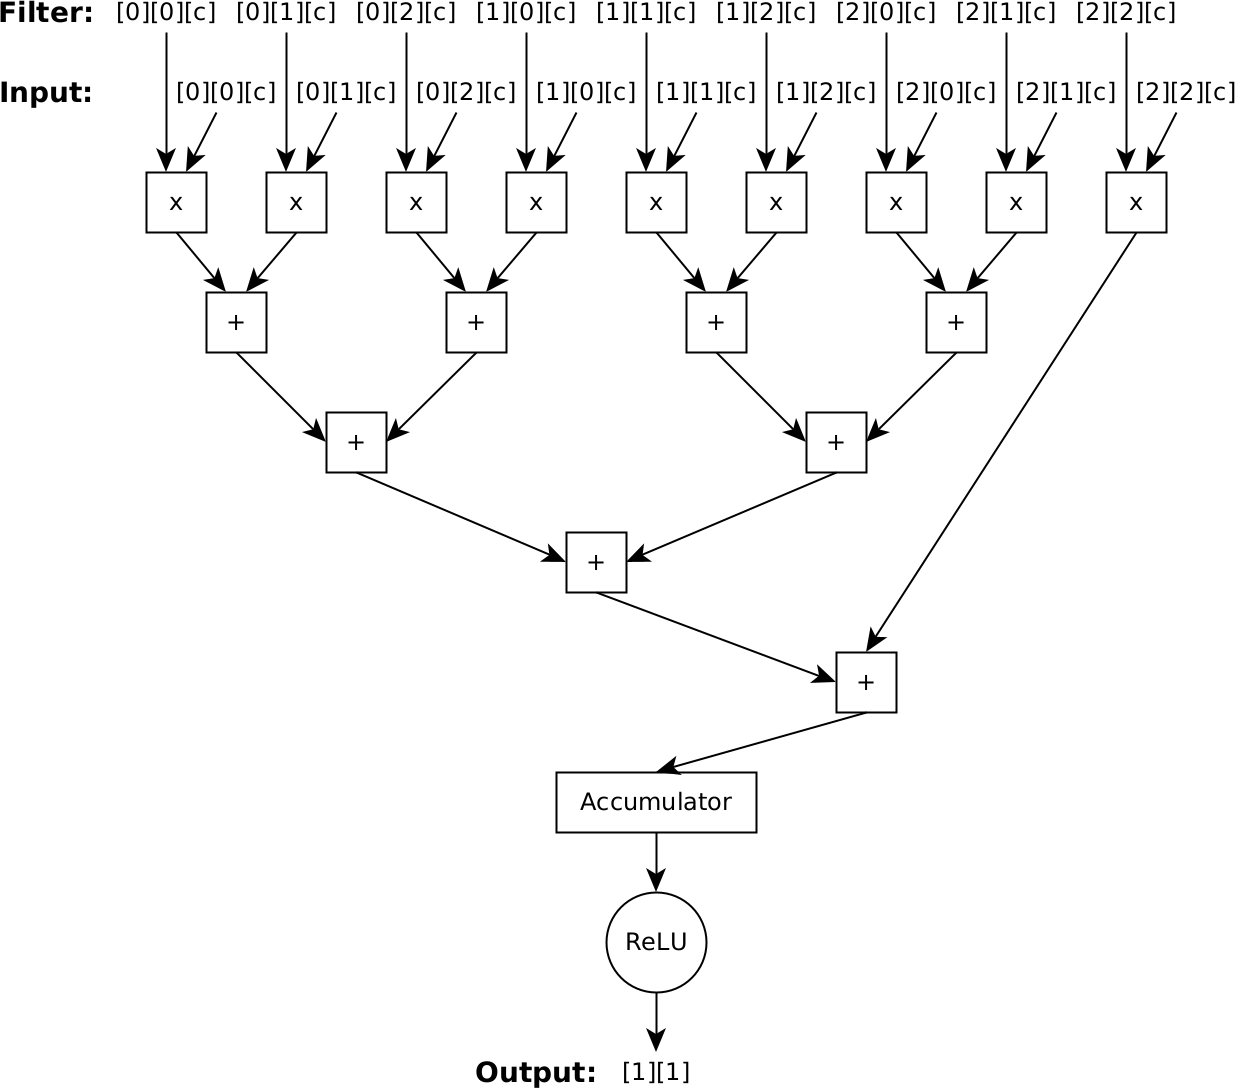
\includegraphics[width=1\textwidth]{Images/Diagrams/conv_mc_order_calculations.png}
            \caption*{Conv2D: order of calculations}
    	\end{figure}%
	\end{minipage}%
	\begin{minipage}{0.6\textwidth}
    	\begin{itemize}
    	    \item Multiple input channels operate additively, accumulator required
    	    \item Reordered Calculations to fit hardware better
    	    \item Floats are not commutative, tiny difference in results
    	\end{itemize}
	\end{minipage}%
\end{frame}



% \begin{frame}{FPGA-based CNN implementation - 2D Max Pooling Layers -  Access Pattern}
% 	\begin{minipage}{0.5\textwidth}
%     	\begin{figure}[H]
%             \centering
%     		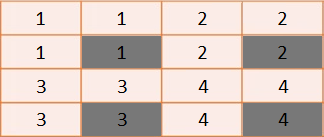
\includegraphics[width=1\textwidth]{Images/Diagrams/maxp_access_patern_on_image.png}
%             \caption*{Data access pattern of max pool}
%     	\end{figure}%
% 	\end{minipage}%
% 	\begin{minipage}{0.5\textwidth}
%     	\begin{itemize}
%     	    \item Input pixels are accessed serially
%     	    \item Two dimensional filters with non-serial access pattern
%     	    \item Data is not reused
%     	\end{itemize}
% 	\end{minipage}%
% \end{frame}



\begin{frame}{FPGA-based CNN implementation - Dense Layers}
    Two components: matrix multiplication and an activation function.

    Dense Layers require all inputs to produce an output. They operate as barriers!
    
    All data before them have been produced. If any of them skips them, must be stored in memory.
\end{frame}

\begin{frame}{FPGA-based CNN implementation - Gradients Calculation Pipeline}
	\begin{minipage}{0.25\textwidth}
    	\begin{figure}[H]
            \centering
    		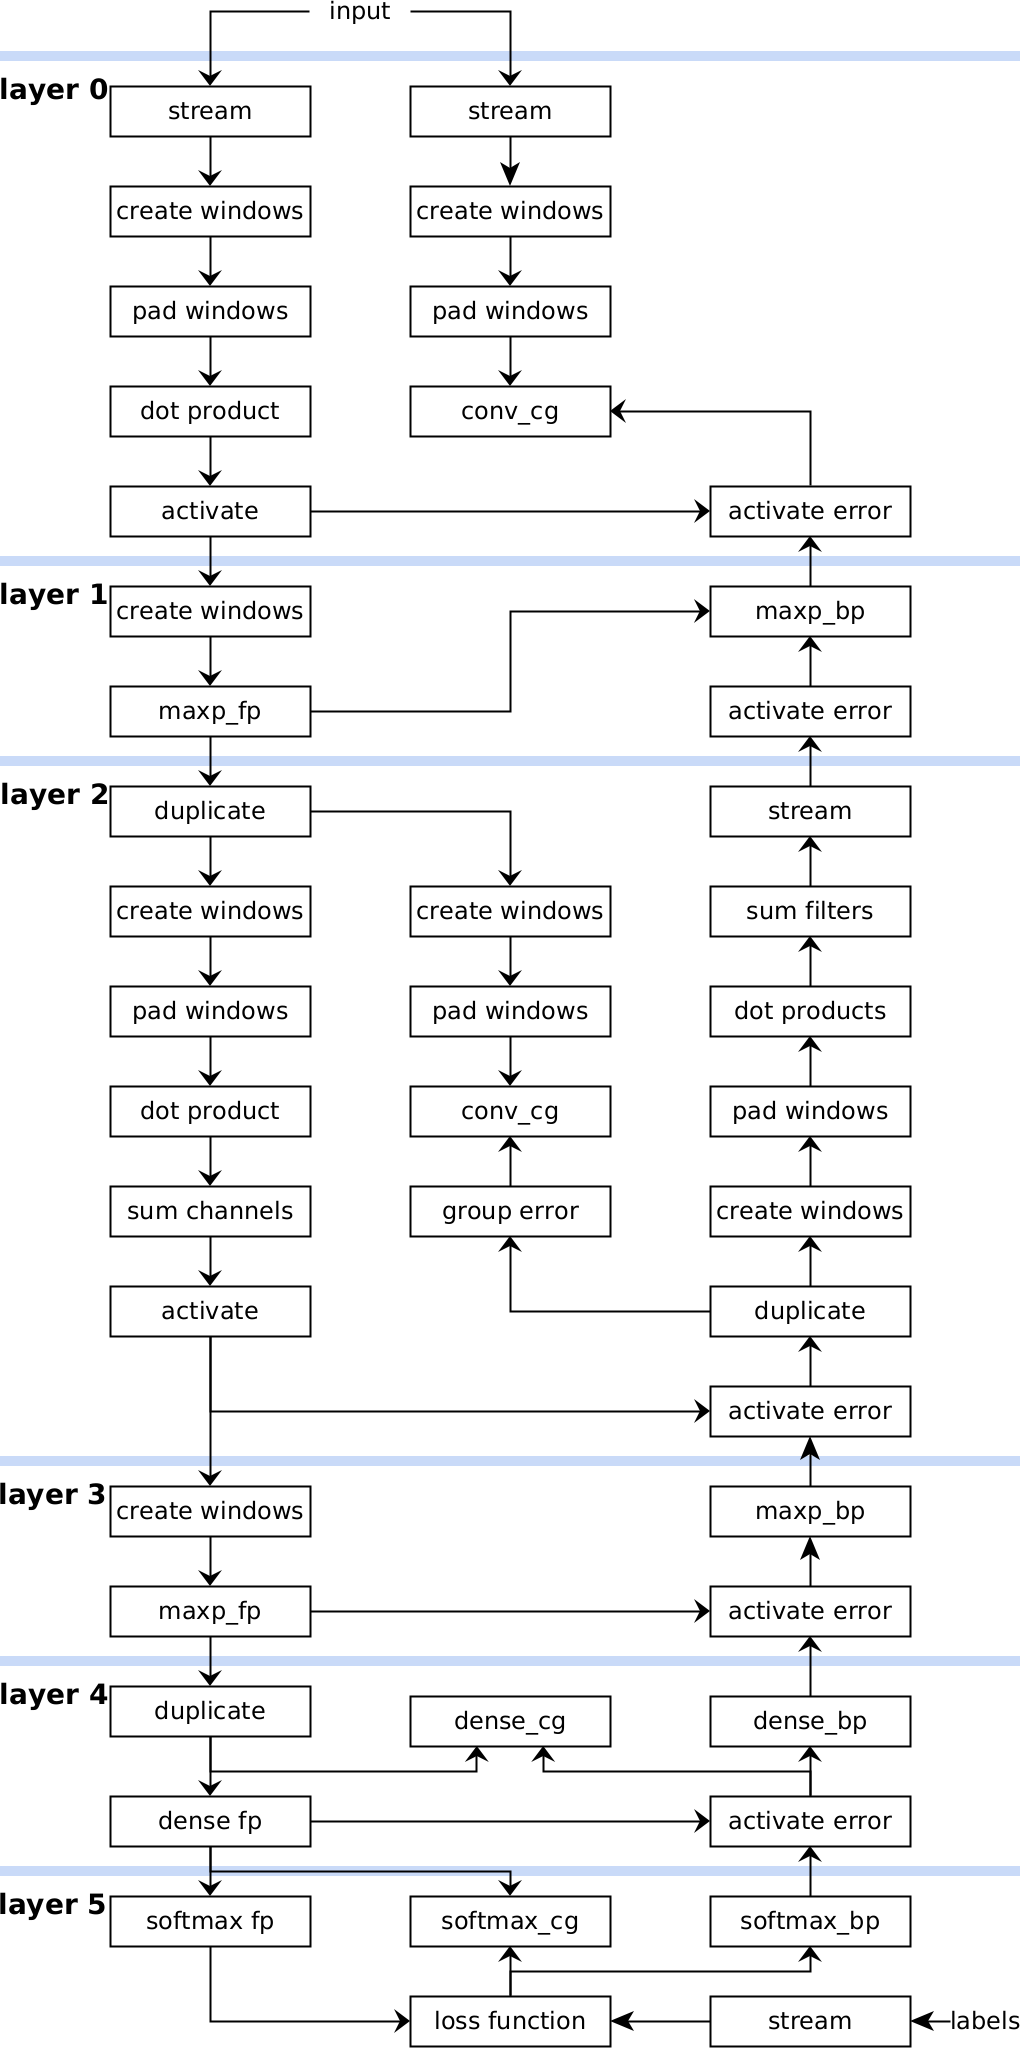
\includegraphics[height=0.8\textheight]{Images/Diagrams/process_batch.png}
    	\end{figure}%
	\end{minipage}%
	\begin{minipage}{0.75\textwidth}
    	\begin{itemize}
    	    \item Dataflow pipeline, hardware functions can run simultaneously
        	\item The Softmax layer split the pipeline to two region that can not operate simultaneously for a single image.
        	\item Inputs are accessed twice, special treatment required
        	\item First Layer does not require back-propagation
        	\item Most hardware functions are data transformations
        % 	\item Free running pipelines to reduce stalls and deadlocks
    	\end{itemize}
	\end{minipage}%
\end{frame}

\begin{frame}{FPGA-based CNN implementation - Batching Inputs}
	\begin{minipage}{0.5\textwidth}
    	\begin{figure}[H]
            \centering
    		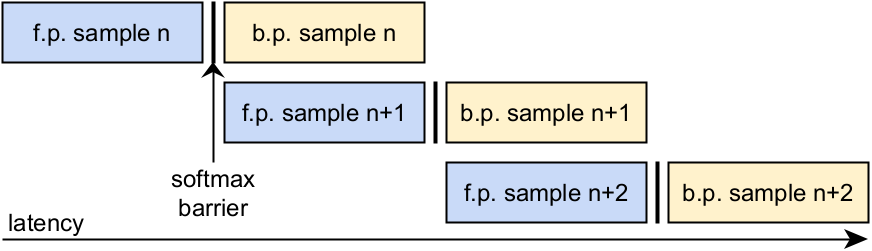
\includegraphics[width=1\textwidth]{Images/Diagrams/pipeline_under_batching.png}
    	\end{figure}%
	\end{minipage}%
	\begin{minipage}{0.5\textwidth}
    	\begin{itemize}
    	    \item The effect of the barriers can be removed by batching inputs.
    	   % \item The function with the highest latency dictates total latency.
    	    \item Vitis HLS trivialize implementation.
    	\end{itemize}
	\end{minipage}%
	
	Data that skips layers may be produced by the forward propagation of the second image, before they are consumed by the back propagation of the first one!
	
	Each sample adds latency equal to the function with the highest latency.
	
	The time between the start of the pipeline and the first time the barrier is reached, is referred as pipeline wind-up latency.
\end{frame}

% \begin{frame}{FPGA-based CNN implementation - Updating Variables}
%     Distinct pipeline
    
%     Gradient Descent with momentum
    
%     All variables are independent to each other
    
%     Parallelism is governed only by latency and hardware usage!
% \end{frame}

\begin{frame}{FPGA-based CNN implementation - Top Function}
	\begin{minipage}{0.25\textwidth}
    	\begin{figure}[H]
            \centering
    		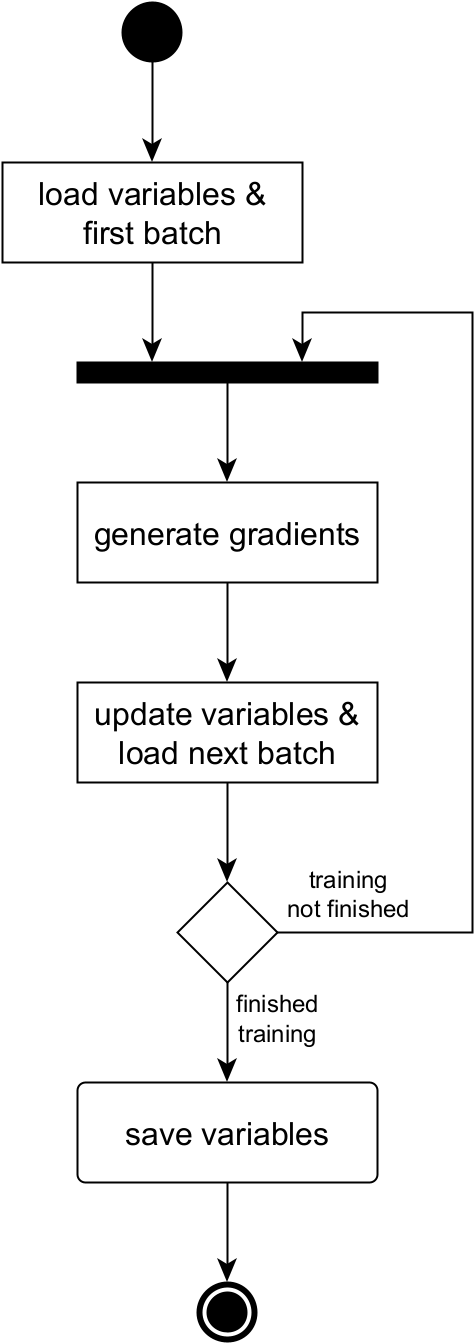
\includegraphics[height=0.8\textheight]{Images/Diagrams/accel_top.png}
    	\end{figure}%
	\end{minipage}%
	\begin{minipage}{0.75\textwidth}
    	\begin{itemize}
        	\item Data that have a life-cycle over a pipeline repetition, require initialization
    	    \item Distinct pipeline to update variables
            \item The pipelines loop for the number of batches
            % \item Save variables moves the final local model to the Global Memory.
    	\end{itemize}
	\end{minipage}%
\end{frame}

% \begin{frame}{Host Program}
%     Driver utilizes XRT API to manage the global memory and run the accelerator.
    
%     The local dataset is moved to Global Memory during initialization.
    
%     The global model must be moved at the start of every GE.
    
%     Incorporating the driver to the FL client is trivial, it is designed to use the same function signatures as the TensorFlow implementation.
% \end{frame}

\begin{frame}{Embedded Systems Perspective}
% 	\begin{minipage}{0.6\textwidth}
    	\begin{figure}[H]
            \centering
    		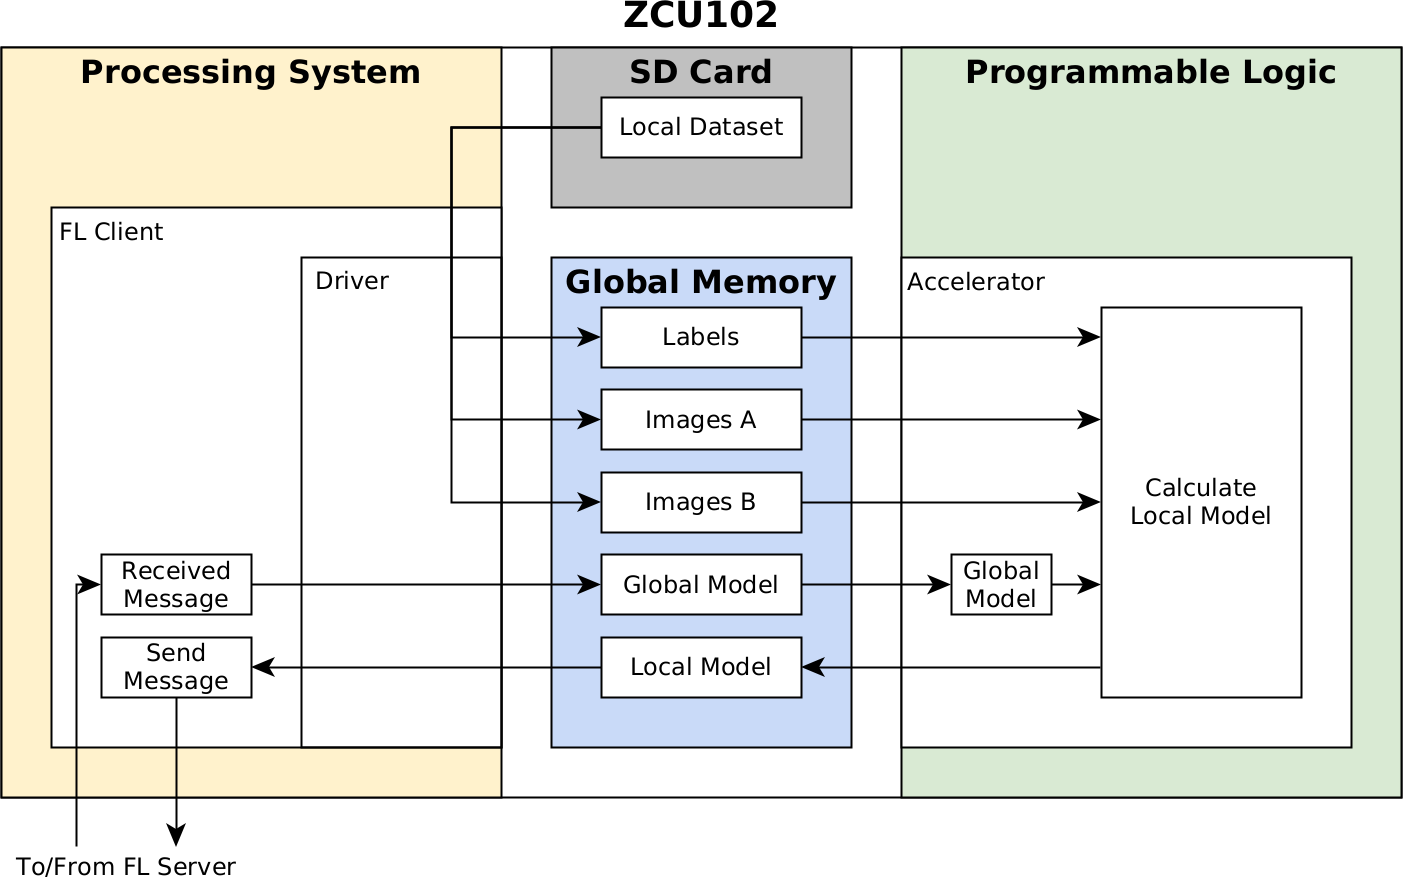
\includegraphics[height=0.8\textheight]{Images/Diagrams/zcu_FL_client.png}
    	\end{figure}%
% 	        FL client from chapter 4\\
% 	        Using Linux sockets\\
% 	        Driver (XRT) manages Global Memory \& Accelerator\\
% 	        Accelerator created with HLS\\
% 	\end{minipage}%
\end{frame}